%!TEX root = ../thesis.tex

\graphicspath{{Chapter6/Figures/}{Chapter6/Tables/}{Chapter6/Charts/}}

\chapter{Discussion}
\section{Introduction} %Section - 6.1 
This chapter is organised into five sections as illustrated in Figure ~\ref{fig:chapter6overview}. Section 6.2 reviews the thesis objectives, hypotheses and research questions relative to the contribution of this research. Section 6.3 reviews the contributions to knowledge contained within this research. Section 6.4 details the limitations of this work in the context of the threats that they pose to the validity of this research. Section 6.5 is a brief summary of the distilled conclusions of this thesis. Section 6.6 considers some of the personal reflections of the author upon this work and the state of the art. Finally, Section 6.7 documents future avenues of research within the field of mining software repositories.

\begin{landscape}
\begin{figure}[htbp!] 
\centering    
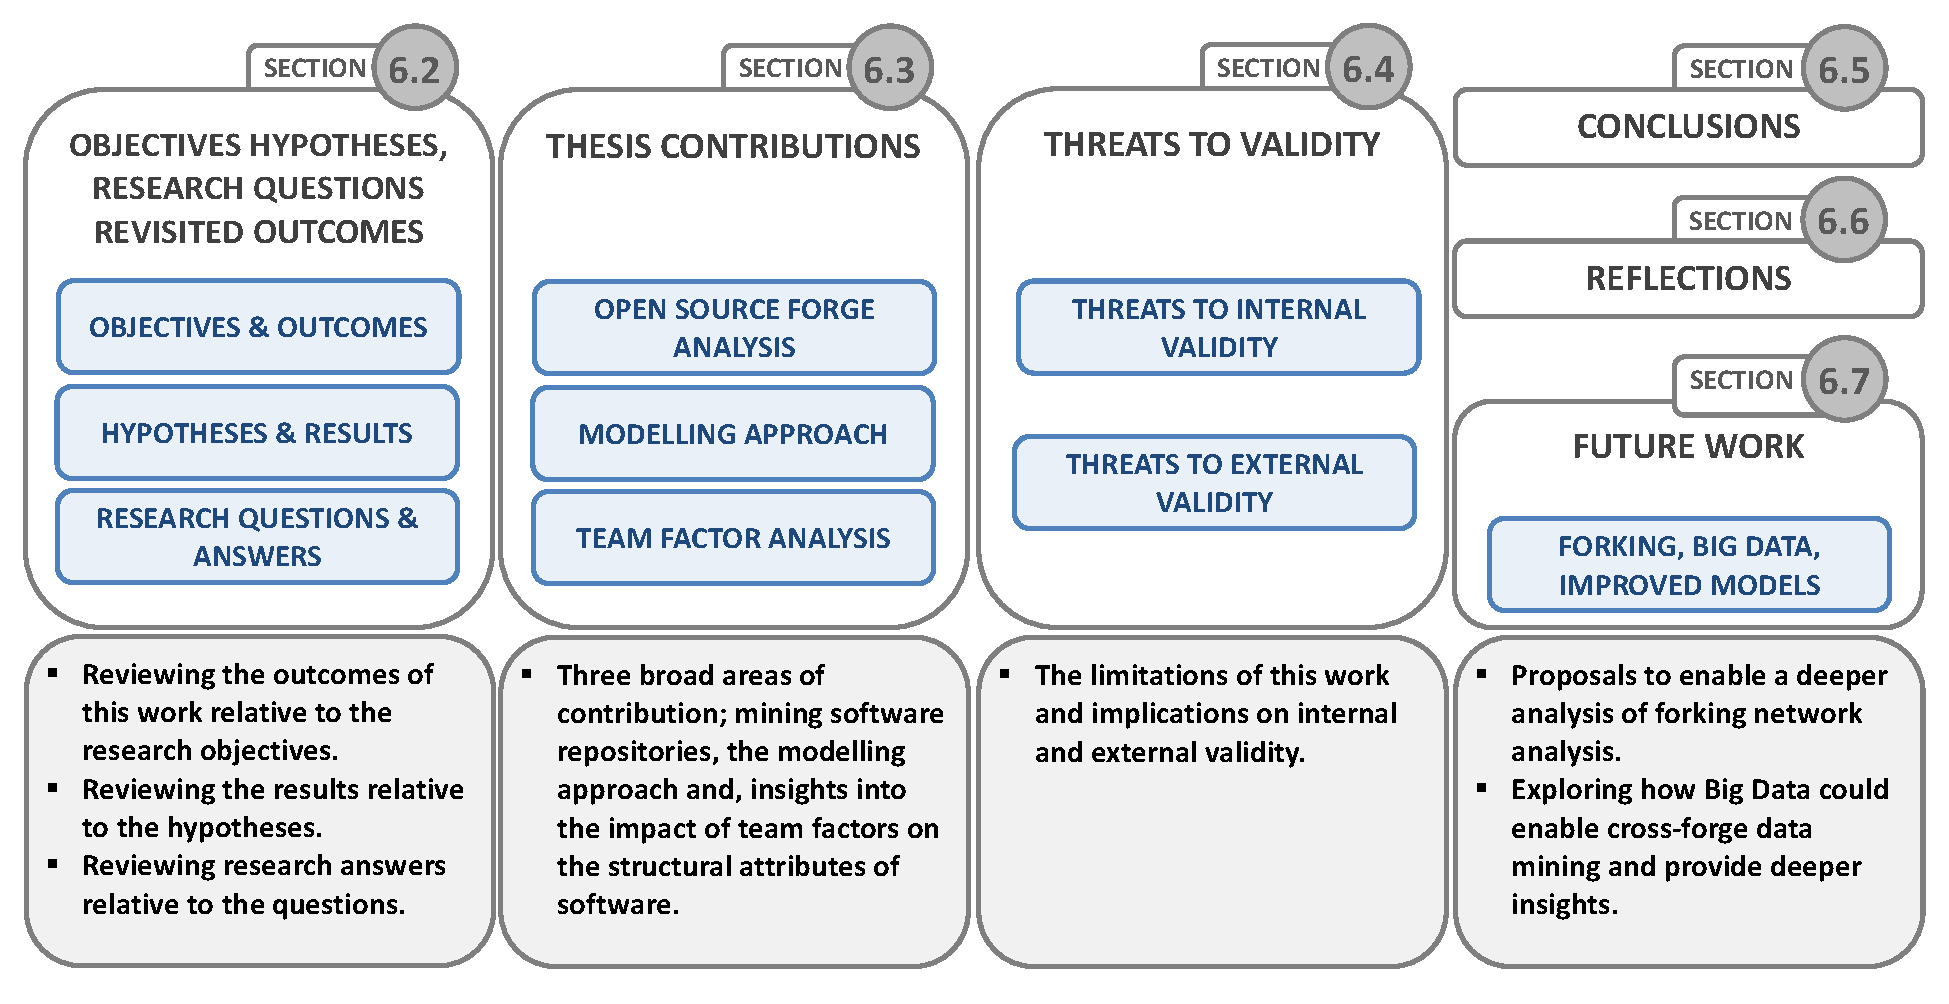
\includegraphics[width=1.3\textwidth]{ChapterOverview.pdf}
\caption{Chapter 6 outline providing an overview of the contents of each section.}
\label{fig:chapter6overview}
\end{figure}
\end{landscape}

\section{Objectives, Hypothesis, Research Questions Revisited} %Section - 6.2
In this section the objectives, hypotheses and research questions are reviewed, assessed and discussed relative to the outcomes in the thesis.

Table ~\ref{tab:ObjectiveOutcome} shows a restatement of the objectives of this research assessed against the outcomes discussed in this thesis. Broadly the research objectives have been met and the results clearly show a relationship between the team factors and the internal and external attributes of the software. 

\begin{table}
\captionof{table}{Summary of objectives and outcomes.}
\begin{tabular}
 \centering 
 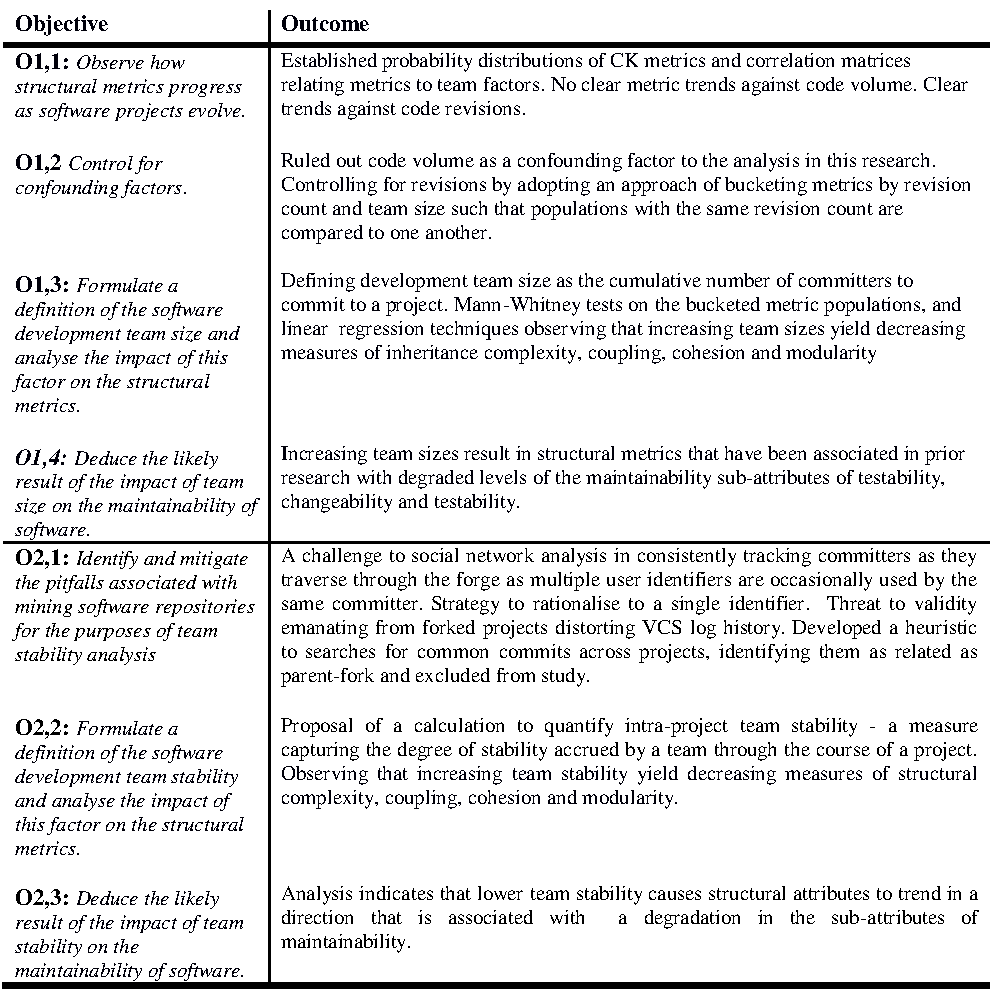
\includegraphics[width=1.0\textwidth]{ObjectiveOutcome.pdf}
 \label{tab:ObjectiveOutcome}
\end{tabular}
\end{table}

Table ~\ref{tab:HypothesisResult} summarises how the hypotheses formulated at the outset of this research mapped onto the results. The alternative hypotheses around the development team size analysis (H1,1.1, H1,1.2) stated that larger development teams would produce software with essentially degraded structural attributes resulting in degraded maintainability. The rationale of the hypothesis was based on the prior work of Nagappan et al., Caglayan et al., Mockus and Bell et al., all of whom observed that there was a negative correlation between development team size and fault-proneness \citep{nagappan2008influence, mockus2010organizational, bell2013limited, caglayan2015merits}. Given that fault-proneness and structural metrics are correlated, and in the absence of any code-level insights, it was considered a plausible hypothesis that all structural attributes of software and team size would show a similar correlation which would be indicative of lower maintainability. 

The results showed that those attributes that had been established to correlate to fault-proneness - coupling, cohesion, modularity - did, indeed, show degradation as team sizes increased. This was consistent with prior research and a confirmation of the alternative hypothesis. The drivers behind trends of degraded coupling and cohesion could be hypothesised to be attributable to the difficulties of effective communication in a larger team leading to developers with conflicting design patterns or alternate approaches causing degraded structural attributes. Through qualitative analysis and engaging development team members, the research community could shed more light as to the drivers behind the trends revealed in this study.

The alternative hypotheses (H1,2.1, H1,2.2) that less stable teams exhibit degraded structural metrics and lower maintainability was based on research by Huckman et al. that found that greater team stability resulted in lower fault-proneness and higher budget adherence \citep{huckman2009team}. The rationale then followed, as with the previous alternative hypothesis (H1,1.1), that this was caused by a general degradation in the internal structural attributes of the software. Higher inter-team and intra-team stability was found to be linked to higher measures of cohesion and modularity, and lower measures of coupling and inheritence complexity. Again, through engaging development team members through surveys in conjunction with a detailed analysis of individual commits, further insights could be gained into the factors driving these observations.

\begin{table}
\captionof{table}{Summary of null hypotheses and results.}
\begin{tabular}
 \centering 
 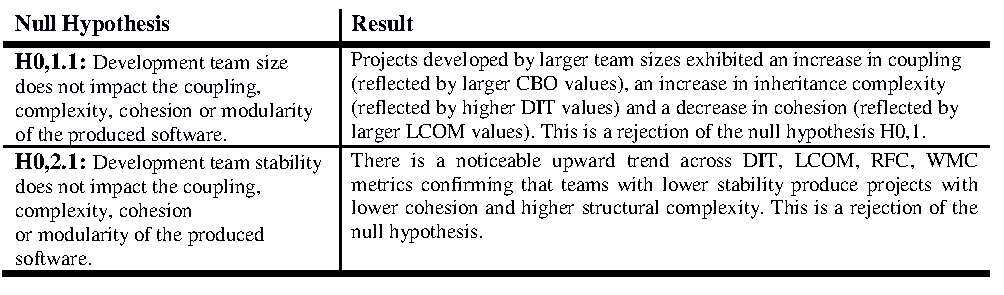
\includegraphics[width=1.0\textwidth]{HypothesisResult.pdf}
 \label{tab:HypothesisResult}
\end{tabular}
\end{table}

Table ~\ref{tab:QuestionAnswer} summaries the headline results against each of the research questions. Broadly speaking, smaller development team sizes and greater team stability result in software with enhanced structural attributes. However, larger team sizes were found to be linked to lower functional complexity which is also associated with enhanced maintainability.

\begin{table}
\captionof{table}{Summary of research questions and answers.}
\begin{tabular}
 \centering 
 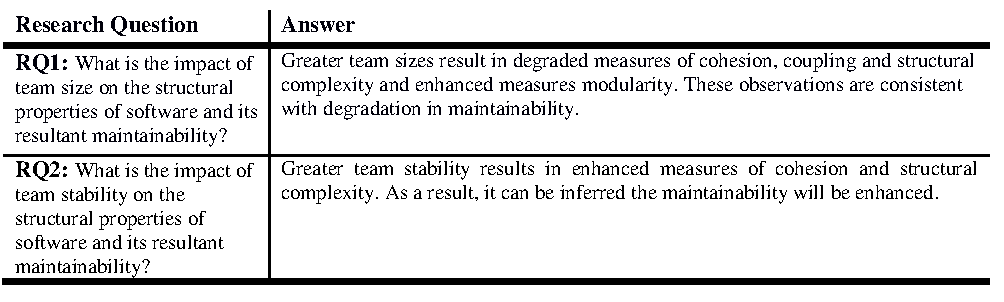
\includegraphics[width=1.0\textwidth]{QuestionAnswer.pdf}
 \label{tab:QuestionAnswer}
\end{tabular}
\end{table}

\section{Thesis Contributions} %Section - 6.X
The contributions in this work span three broad areas; furthering the art in the field of mining software repositories, the unique aspects of the linear modelling approach in this thesis and, finally, insights into the impact of team factors on the structural attributes of software.

\subsection{Open-Source Forge Analysis}
As discussed in the 'Related Work' chapter, the practical challenges of mining open-source forges is well documented in existing research. Thematically this work covers tooling, pitfalls and insights from the perspective of researchers. Separately to this there is work that performs static analysis on selected open-source projects and, also, extracts insights which can help process improvement in some fashion. This research focuses on a single open-source forge and spans both of these areas of research with several specific contributions.

\begin{itemize}
\item  \textbf{GoogleCode forge  analysis: } This research studies an entire forge revealing several insights which go to a greater level of granularity than existing open-source forge research which tends to derive insights at the forge and project level \citep{howison2009flossmole, iqbal2012integrating, squire2017lives}. Committer behaviour across the forge was studied as it informed the approach to the team size and stability analysis. It was possible, through this, to establish the population of unique committers (identity reconciliation challenges notwithstanding as documented in Section 5.2.1) and track their activity throughout the history of the forge. This enabled observations on the number of projects that committers contribute to as well as the nature of their contributions (number of commits, number of files per commit and timeframes of activity). With this information it was possible to identify where committers collaborated on multiple projects, crucial to the team stability sample identification. 

This was a one of many potential use-cases for this type of data set and social network analysis in open-source is an active field of research with plenty of other use-cases \citep{hassan2008road, hemmati2013msr}. For a representative sample of the forge it was then possible to mine structural metrics and join those observations to the commit meta-data (through the definition of a relational database schema). Through studying observations from 173,190 class files in the team size sample it was confirmed that CK metrics from projects of this forge follow heavily skewed non-normal distributions in-line with the work of Succi et al. and Basili et al. who had conducted their research on a smaller disparate data sets \citep{basili1996validation, succi2005empirical}. The reported moderate collinearity between each of CBO (capturing cohesion and modularity) RFC and WMC (capturing structural complexity) was also confirmed.

\item  \textbf{Identifying forked projects: } Forking presents a number of perils when not properly considered. These perils can affect researchers extracting insights by mining VCS histories, developers identifying projects to contribute to and end-users looking to utilise a project artefact. This research is concerned with the first use-case and has, for the first time, highlighted forking as a threat to the validity of network analysis in open-source forges. Existing research focusses on project forking for the purposes of studying the its motivations and outcomes \citep{robles2006mining, nyman2011fork}. This research presents an approach to the automated identification of forks avoiding the costly code clone analysis proposed by Ray and Kim \citep{ray2012repertoire} and relying solely on VCS logs which are much less costly to mine.

The approach presented was practically applied to mining the entirety of the GoogleCode forge and the threat to validity that forking poses was quantified with 6.25\% of projects in the forge found to be forked and therefore showing commit history which is misleading when taken out of context. The approach presented is not limited to GoogleCode but can be generalised to all forges which use SVN or GIT as their underlying VCS.
\end{itemize}

\subsection{Modelling approach}
There are several noteworthy aspects to the nature of the linear models used to capture the trends observed in the GoogleCode forge that constitute a contribution to knowledge.

\begin{itemize}
\item  \textbf{Modelling CK metrics as a dependent variable: } Existing research casts CK metrics as the \textit{independent} variable and models their relationship with the externally observable attributes of software as documented extensively in the related work sections 2.3.3-2.3.4. Within this research, for the first time, these CK metrics are treated as the \textit{dependent} variables and the impact of team factors on these variables are modelled. This type of analysis allows existing models to be brought to bear in order to deduce the likely impact of these team factors on the externally observable attributes of software. For instance, this research concludes that LCOM has a positive linear relationship with team size. Bruntink et al. and Badri et al. both found LCOM to be an inverse predictor of testablity \citep{bruntink2006empirical, badri2011empirical}. It is therefore it is reasonable to suggest that team size is likely to have an inverse relationship with the testability of the produced software. 

Through this modelling approach, it was discovered that revisions are a confounding factor when studying the impact of team factors on CK metrics. This complements both the work of Emam et al. and Zhou et al. who found that controlling for size was essential when modelling CK metrics as the \textit{independent} variable  \citep{el2001prediction, zhou2006empirical}.

\item  \textbf{Definition of team stability: } Huckman established a general approach to measuring team stability using the cumulative time that team members worked together \citep{huckman2009team}. In this thesis the Huckman approach was transposed onto a quantitative measure of stability that can be derived through the analysis of VCS logs alone, lending itself to open-source forge studies. This work presented a distinction between \textit{intra}-project  and \textit{inter}-project stability; respectively the stability accrued through the course of an individual project and that gained through the collaboration of the project team on multiple projects. Intra-project stability was captured through the formulation of  the Lack of Stability Ratio (LSR) and the practical application of this measure to a representative sample from the GoogleCode forge was documented within this thesis.
\end{itemize}

\subsection{Team Factor Analysis}
At the core of this thesis lies the established relationship between the team factors of size and stability and the structural metrics of software.

\begin{itemize}
\item  \textbf{Team size trends: } Prior research established team size as a key determinant of project success with models finding a relationship between team size and both lower productivity and increased fault-proneness. This thesis contributes to the art by also establishing team size as a significant predictor to CK metric values, shedding light on the potential underlying effects that drive the externally observable attributes. Both the correlation analysis and the linear models showed a positive relationship between team size and all metrics with the exception of NOC. The effect of team size was particularly marked in DIT and LCOM with team size accounting for almost half the variance in these metrics. This work applies linear mixed models to a multi-project metrics study for the first time finding a strong idiosyncratic 'project-specific' aspect that outweighs the team size effect. Given the models summarised in Table 2.4, this implies an inverse relationship between team size and the sub-attributes of maintainability which is generally consistent with the prior art in the field. 

\item  \textbf{Team stability trends: } Huckman et al. studied a dataset comprising over 1000 projects and found that increased team stability yielded lower fault-proneness. Through the course of this thesis it was established empirically that there is a positive correlation between a \textit{lack} of team stability and CK metrics which, in turn would be associated with a deterioration in the sub-attributes of maintainability and fault-proneness. Through the discovery of these trends this work sheds a light on the underlying effects that could potentially have driven Huckman's observations (or indeed those of Gardner et al. who found that increased team stability was linked to an increase in client satisfaction \citep{gardner2012dynamically}).
\end{itemize}

\section{Threats to Validity} %Section - 6.5
This section covers the internal and external threats to validity affecting this research.

\subsection{Threats to External Validity}

\begin{itemize}
\item  \textbf{Development models} Open-source projects tend to have a particular dynamic which sees a limited number of core contributors taking a central role while the majority of contributors take a peripheral role and do not engage in projects for extended periods of time \citep{howison2006social}. This can contrast with commercial software which often is developed by a relatively engaged development team. In either development approaches there could core contributors who act as gatekeepers into the version control system and mandate a review and approval process prior to any commits becoming part of the main source code repository. It can be hypothesised that this could ultimately impact the structural attributes of the software. For instance, a central core of experienced committers with a good knowledge of the system could provide guidance on component reuse where such opportunities may otherwise have not been exploited. Within the GoogleCode repository there is no project meta-data that can be exploited to inform on these factors.

\item  \textbf{Physical locations} Brooks posits that larger teams face greater difficulties in communication compared to smaller teams and hence productivity is impacted. However, one significant factor that influences the efficiency of communication is the physical location of the members of a team. Teasley argues that collocating a team can double productivity \citep{teasley2000does}. Factoring in the physical setup of the development teams contributing to the studied projects is beyond the scope of this research.

\item  \textbf{Development languages} It is important to re-state that this research only takes into account observations that can be made of Java code, to the exclusion of all other languages. It is possible that there may be factors that cause particular trends that are observed in Java software to be absent from software developed in other object-oriented languages. It could be argued that, as the results observed in this study are generally consistent with the vast body of research (research which does span multiple OO languages such as C++, Java and Smalltalk), it is unlikely to be a significant threat to validity. However, nonetheless caution should be exercised when applying the lessons learnt in this study to projects written in other languages.

\item  \textbf{Generalisation to other forges} While this work uses a large data set (certainly in comparison to similar studies) there was no attempt to establish how the forge chosen for this study, GoogleCode, could differ in nature to other forges. While there is no indication that GoogleCode is, indeed, biased towards any particular influencing factor, it cannot be ruled out as a threat to validity. It is also worth noting that, while this work succeeded in observing broad trends across the forge, it is noted that not all projects within the samples followed these trends. There are a number of factors that can impact the structural attributes a particular project, not captured in this study, and which may affect the generalisation of this work.
\end{itemize}

\subsection{Threats to Internal Validity}

\begin{itemize}
\item  \textbf{Linking structural attributes to external attributes} Part of this research is to infer the impact of the observations made of the structure of software on its externally observable attributes. This inference draws on the work of prior researchers who have established correlations between metric values and aspects of maintainability. For that reason, any inferences drawn in this work inherit the threats to validity in that prior research. Where we link CK metric observations to external attributes of understandability and changeability, it is necessary to state the limitations of the research conducted by Harrison et al, whose work first established correlations between metric values and these external attributes; namely that their use of small student projects as a data set constitutes a threat to validity when applying these results to larger commercial or open-source projects \citep{harrison1998investigation}. Likewise Bruntink and van Deursen, whose work established correlations between CK metrics and testability, note that their criteria for evaluating testability may not be applicable to all projects \citep{bruntink2006empirical}.

\item  \textbf{Functional nature of projects} This threat to validity concerns the mix of server-side and client-side programming that exists, particularly, in those projects with a User Interface (UI). Best practices dictate that the UI should be a thin layer with the business logic existing in a server-side service layer. In a typical Java project, the server-side programming would be in Java while the client side could be in any one of a number of scripting languages such as JavaScript. As this UI layer is not studied in this research, there is a 'blind spot' whose size could vary according to degree of adherence to best practices. For instance, if larger teams tend to adhere to the principle of 'separation of concerns' to a greater degree than smaller teams, it could be that greater complexity observed in the server side is incorrectly attributed to the larger teams while, in fact, that complexity also exists in the smaller team's work - only that it exists in the client-side scripting code. This is depicted, in basic terms in Figure ~\ref{fig:ContrastingSystems}.

\item  \textbf{Team sizing model} The project comparison analysis in Chapters 4 and 5 showed that, while we attribute a single figure to the size of a development team based on the cumulative number of project committers, the reality of the matter is more nuanced. Individual committers or groups of committers are often responsible for a disproportionate contribution to the project and there is a loss of information when this behaviour is reduced to a single number. In Section 4.1.1 it is argued that the contribution of so-called 'peripheral' committers could not be ignored as they are undoubtedly an influence on the codebase of a project. However, it can be equally argued that not quantifying or factoring in the nature of the committer contributions does not allow us to draw a potentially important distinction between projects with differing proportions of core and peripheral developers. 

\end{itemize}

\begin{figure}[htbp!] 
\centering
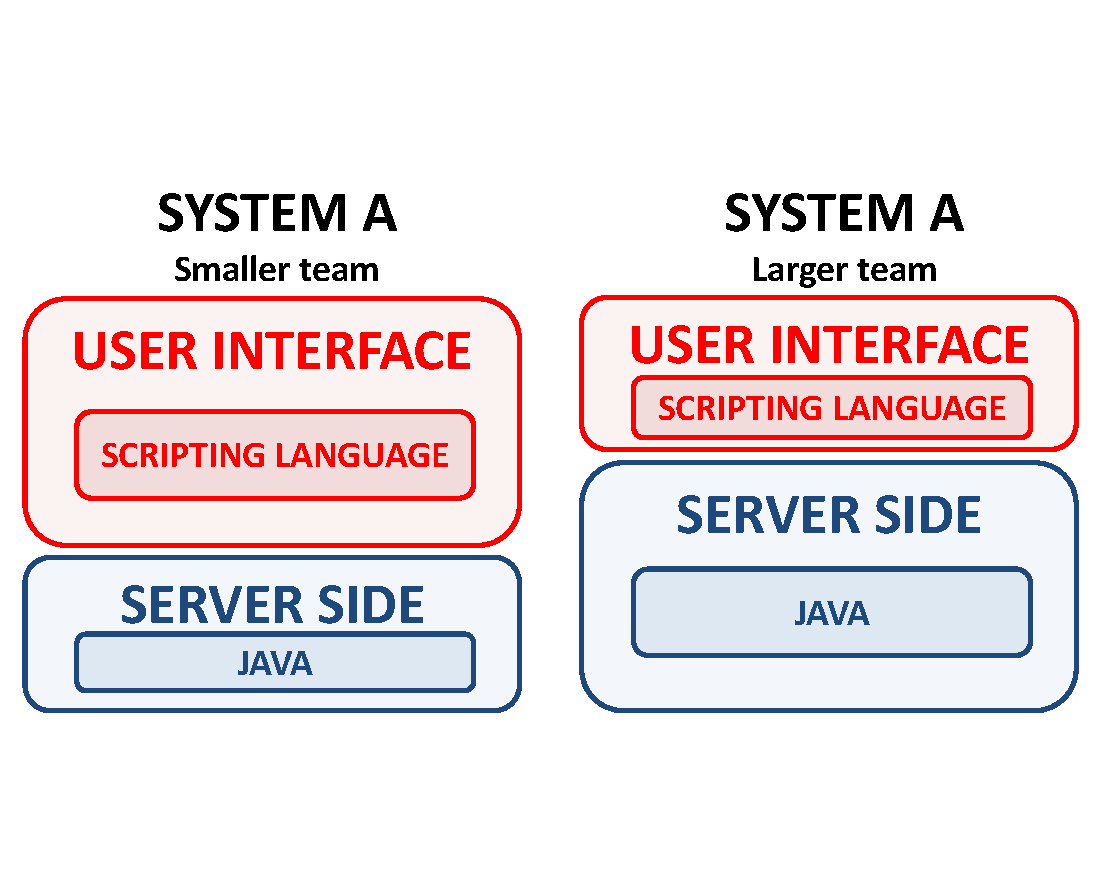
\includegraphics[width=1.0\textwidth]{ContrastingSystems.pdf}
\caption{An illustration of how a larger team could produce software with a greater adherence to the separation of concerns with more of the complexity residing on the server side.}
\label{fig:ContrastingSystems}
\end{figure}

\section{Conclusions} %Section - 6.5
As mentioned in section 1.4 of this thesis, the overarching research problem that this work aims solve for is the difficulty in appropriately sizing and resourcing software development teams to achieve optimal performance and stakeholder satisfaction. It was discussed how organisations often had multiple options available to them in this regard; for instance forming new large teams or seconding existing small stable teams. 

This work helps inform practitioner decision-making by providing greater insight into the impact that team composition can have on the sub-attributes of maintainability. Rather than simply observing a relationship between team factors and externally observable attributes, this work provides an insight into how large or unstable teams lead to the degradation of the internally observable attributes which consequently drive the degradation of externally observable attributes including maintainability. As stated by Fenton and Bieman, practitioners are accustomed to measuring and monitoring internal attributes throughout the development process \citep{fenton2014software}. Internally observable attributes of software can be measured and monitored in real-time through tools such as Sonar enabling practitioners to monitor and mitigate risks that may arise from unstable or large teams \citep{sonar}.

While the focus on team size and stability provided insights that it is hoped will be of value to both the research community and practitioners, there were other significant contributions within this work. A methodology was put forward to enable the study of externally observable attributes of software through the internal structural attributes of software, leveraging existing research to tie both strands together. In doing so, practitioners can focus on specific, measurable structural attributes as a mitigation strategy against some of the observed negative trends that can result from team factors. Furthermore, this work brings relevance to existing research. By way of example, Chidamber et al. \citep{chidamber1998managerial} find that higher measures of coupling and lower levels cohesion are indicators of lower productivity, greater rework and design effort. These structural attributes are side-effects of larger team sizes, so it is reasonable to deduce that the aforementioned degradation in productivity, rework and design effort are likely to also result from larger teams.

While studying the impact of team factors by studying the GoogleCode forge, many practical difficulties were encountered in mining a large and diverse forge. In particular, performing accurate and reliable network analysis for the purposes of the team stability analysis was particularly challenging and it is hoped that the work in this thesis to mitigate these threats to validity will prove helpful to the broader research community. 

\section{Reflections} %Section - 6.6
The author has a number of personal reflections on this work from the vantage point of both a researcher and an experienced practitioner.

\begin{itemize}
\item  \textbf{Challenges mining open-source forges: } A significant proportion of the effort expended in this work has been in obtaining, cleaning and modelling the data set. This is not unusual; a recent survey of data scientists reported that 70\% of their time is typically spent collecting, labelling, cleaning, organising and modelling data while only 10\% is spent mining data for patterns \citep{crowdflower}. The author was struck by the logistical complexity of mining a large forge despite the clean interface that Version Control Systems expose to make both code and meta-data available. For instance, retreival of revision logs across 236,787 projects necessitated several iterations of the VCS mining scripts in order to parallelise the data retrieval process. It was also necessary to host the mining software on a remote virtual server in order to achieve the requisite download speeds to complete the retrieval process in a sensible time-frame. Similarly, executing network analysis on such a large data set presented it's own challenges in writing the software in a suitably memory efficient manner. Once the data set was sampled and distilled to an easily consumable form, conducting statistical tests was easier than the author had anticipated. This was due, in large part, to the ease of use of data analysis tools such as the Anaconda data science workbench and the many open-source python libraries with their active developer communities \citep{anaconda}.

\item  \textbf{Future roles for machine learning and big data: } The vast quantities of data and meta-data that are available within software repositories are arguably under-utilised and should be leveraged to improve success rates of software projects in industry. As discussed in this thesis, this data could be used to identify, in real-time, potential threats to the externally observable attributes of software. While software metrics have seen some industry adoption, particularly through the use of Sonar  in enforcing so-called 'quality-gates' that commits must pass become part of the software \citep{ampatzoglou2018framework, sonar}, the use-cases of management adoption of  structural metrics remain few and far between. There exists a gulf between the empirical approach to the study of software by the research community and the approach of practitioners which is often less structured and less empirical. One of the aims of this research is to help, in whatever small way, bridge this gap. One key reflection that the author has from this thesis is that driving a more empirically-oriented approach to software development is key to it's continuing maturity as an engineering discipline.

\item  \textbf{Reproducibility of results: } While surveying the prior art, it became evident that reproducibility of results in the field of mining software repositories is a particular challenge. Some academic research draws upon closed-source software, not available to the research community, to research industrial case studies. Even where open-source software is the subject of study, often the literature inadequately documents the methodology; a real hindrance to anyone attempting to validate the work or, indeed, replicate the study to serve as a baseline for their own study. Given the burgeoning interest in data science, the research community would do well to make curated data sets available to the broader community through GitHub or specialised data set sharing and collaboration platforms such as Kaggle to crowd source efforts to uncover insights and help drive greater interest in industry adoption of metrics \citep{github, kaggle}.

\end{itemize}

\section{Future Work} %Section - 6.7
To support the network analysis that drove the team stability analysis, there was effort to establish parent-fork project relationships throughout the GoogleCode forge. This effort was limited to those relationships that had the potential to skew the inter-project team stability analysis and therefore focussed exclusively on those forks that had been established through a direct clone of a repository from within the GoogleCode forge itself. As a separate strand of research, there is value in a broader and more detailed study of forking relationships.
To support this broader study of forking relationships and to also drive a more comprehensive study of open-source developer contributions, it is worthwhile to consider what shape a cross-forge data mining study may take. In this section a Hadoop-based architecture is proposed as a potential solution to analysing the vast data sets that a cross-forge mining effort would yield. 

\subsection{Network Analysis}
When studying open-source repositories, there are a number of perspectives from which data about project forking relationships drive value. Capiluppi et al. proposed  an approach to quantify committer contributions to open-source projects and assign a measure similar to the H-index used in the academic world \citep{capiluppi2012developing}. Any assessment of committer contributions will be skewed if equal weight is assigned to commits that import work from other projects versus a committer's original work.  This is particularly pertinent given that there has been a recent upsurge in the use of open-source repositories such as GitHub for identifying and recruiting software development talent. To a recruiter it is essential that individuals are not being attributed credit for work that is simply imported from other projects as bad hiring decisions can be very difficult to reverse.

Successful projects can garner a large number of forks and occasionally the fork can overtake the parent in popularity such as in the case of Firefox forked from Mozilla and Ubuntu forked from Debian. Clearly there will be some visibility on forks which garner a large amount of activity but many forks fail to make a significant contribution at all. It will remain an open question as to how many forks fail due to a lack of innovation and how many fail simply through lack of visibility in the wider community but we believe that providing visibility on the  alternate development streams would help inform developer and user decision-making. For example, a particular set of customisations present on a fork may make that project more attractive to a certain user community. From a contributor's perspective, a highly productive, yet smaller, developer community may be more attractive to join. According to a recent survey by Jiang et al. 42\% of developers believe that there is value in an automated recommendation tool to assist in choosing repositories to fork \citep{jiang2017and}. 

Based on the lessons learnt from the narrow study of project relationships in this thesis a broader solution is presented that aims to achieve several goals:

\begin{itemize}
\item  \textbf{Plug-in heuristics} The network analysis in the previous chapter used a heuristic based on 'common commits' to identify project forks. That particular heuristic relied on the observation of multiple commits with identical meta-data across projects as evidence of the forking relationship. This heuristic is particularly suited to identifying projects which have the potential to skew VCS based network analysis within a single forge but this is by no means the only useful heuristic in the broader context of mining. By way of example, adding additional mining commit comments or code clone detection will yield a more comprehensive analysis.
\item  \textbf{Directional relationships} The network analysis in this thesis did not look at the directionality of the relationship between related projects. There was no attempt to discern the parent from the fork as this data was not relevant to the mining of 'stable project pairs'. However, from the perspective of a project stakeholder, this information is relevant. A basic heuristic which could be applied to this problem could identify the project with the greatest number of commits as the parent is likely to be the more active project. However there are, of course, exceptions to this norm.
\item  \textbf{Visualisations} While the raw analysis mapping out parent-fork project relationships is a useful input to those looking to conduct detailed network analysis or measure developer contributions, it is not an appropriate output for project stakeholders looking to select a project for adoption as a user or a contributor. For this reason, a visualisation can provide value for complex project network graphs.
\end{itemize}

To solve for these challenges a simple bespoke framework was prototyped which was based on several of the design patterns and components in the toolchain that was presented earlier in this thesis. Figure ~\ref{fig:ForkingUML} presents a UML depiction of the class structure of the implementation. At the top-level a Controller is responsible for reading commit data from the various implementations of CommitLoader - retrieved in the form of the object graph described in the Commit interface and its dependencies - and passes them into the implementations of the Heuristic which returns an instance of Result containing all the projects found to be forked from others. The heuristic interface is flexible enough to allow for the capture of meta-data such as a measure of the code volume of original content within a fork. For visualization, a node network graph renderer can generate visualisations for the node relationships as illustrated in Figure ~\ref{fig:ForkedNetworkGraph}. For this prototype the Arbor.js framework was used as it's open-source and fairly basic, although there are several advanced network graphing tools. 

\begin{figure}[htbp!] 
\centering    
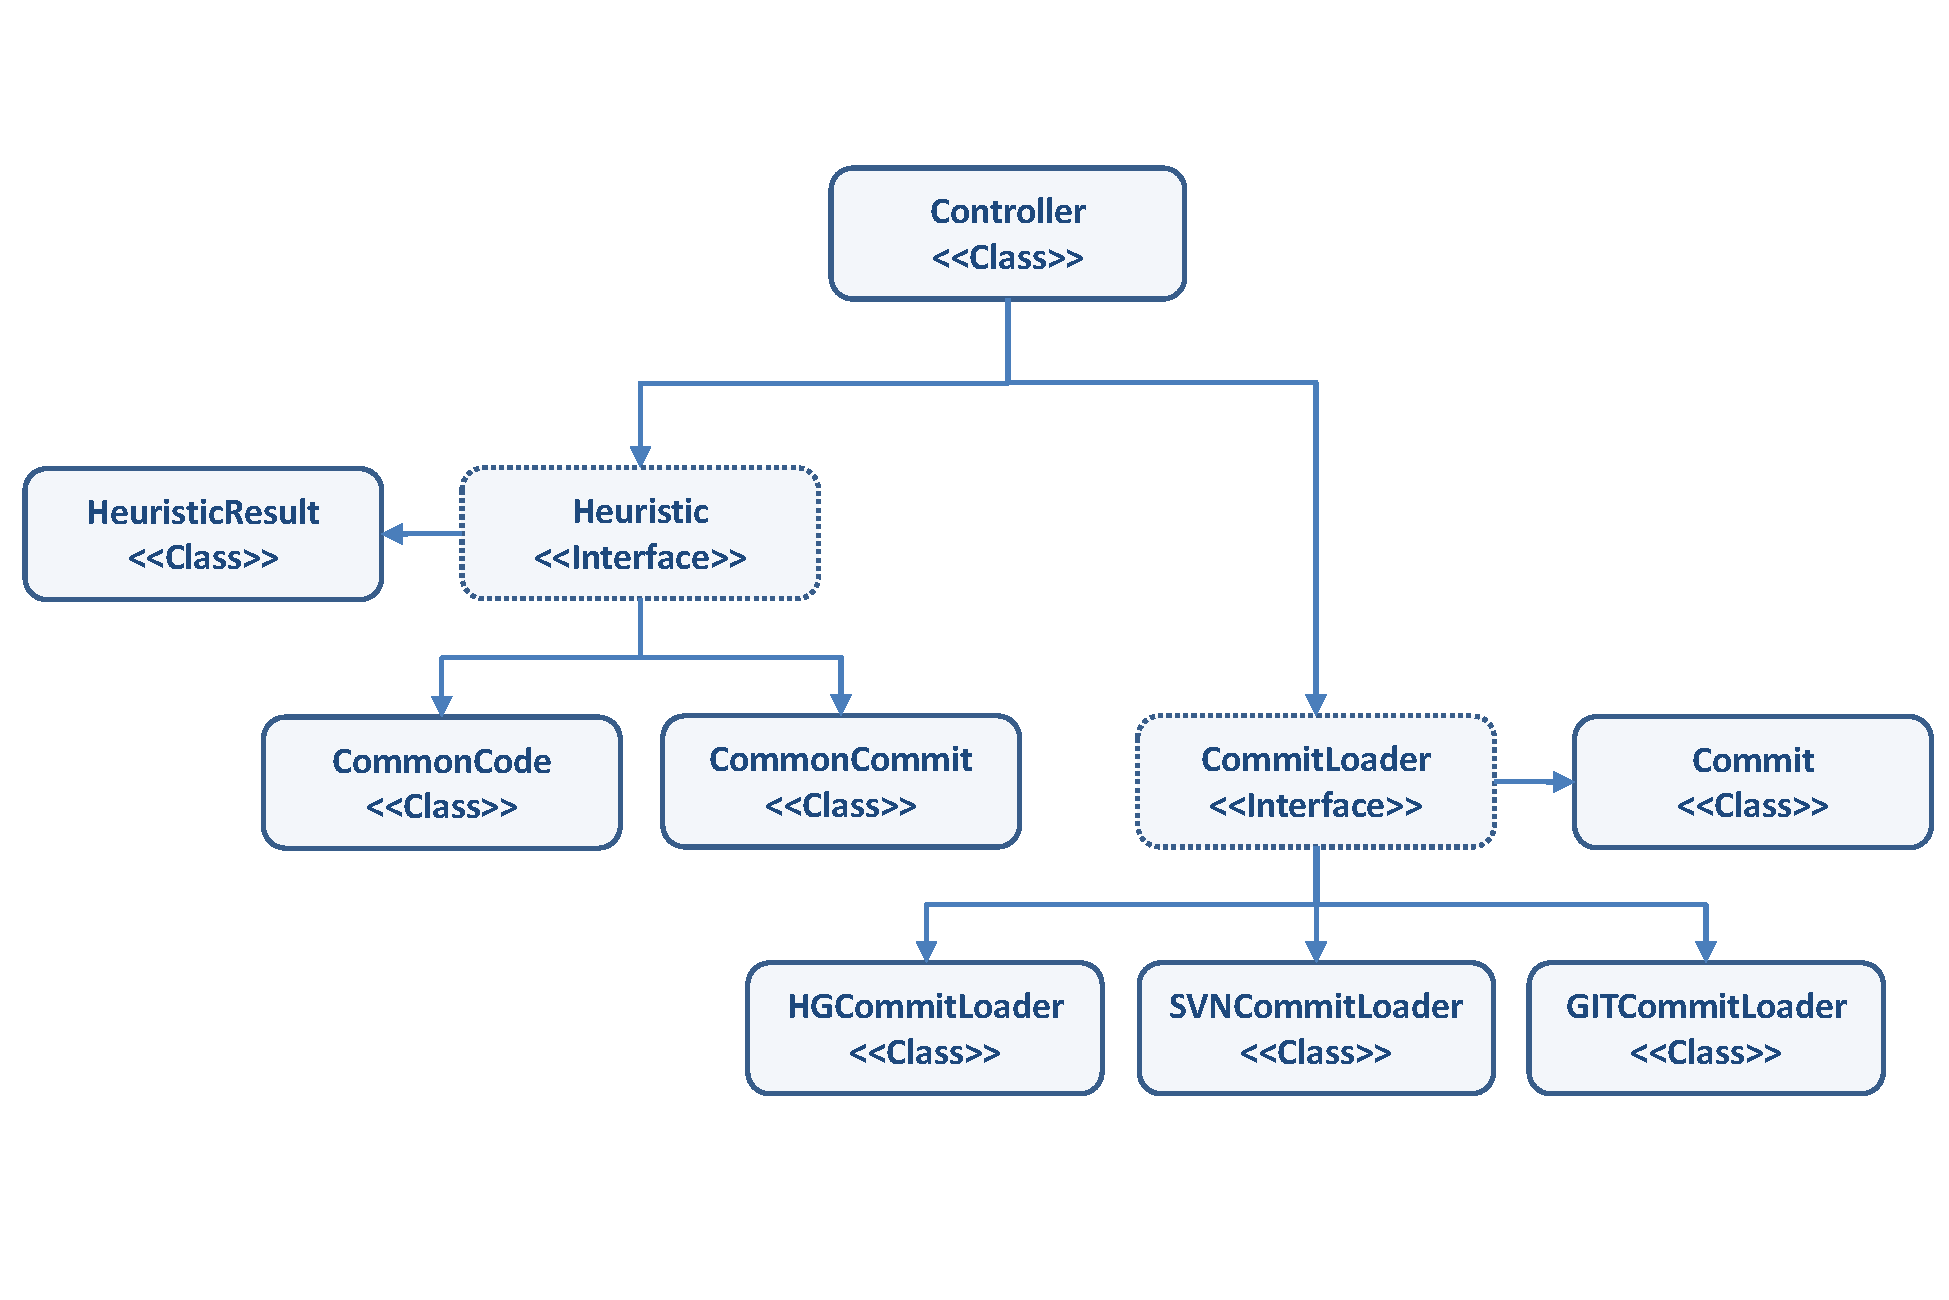
\includegraphics[width=0.9\textwidth]{ForkingUML.pdf}
\caption{UML Diagram illustrating structure of the prototype of heuristics framework}
\label{fig:ForkingUML}
\end{figure}

\begin{figure}[htbp!] 
\centering    
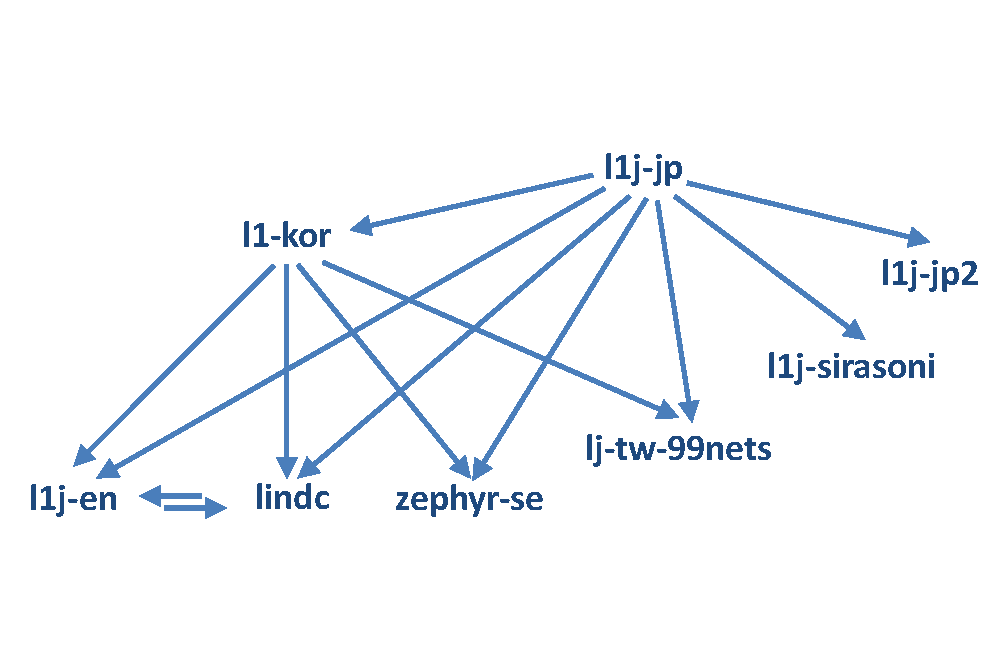
\includegraphics[width=0.8\textwidth]{ForkedNetworkGraph.pdf}
\caption[An example network graph using the example of the Lineage project.]{An example network graph using the example of the Lineage project which is an online multiplayer role playing game which is particularly popular in Korea and Japan. The projects illustrated are mostly language variants of Lineage server emulators. There are a number of additional forks on the periphery of the diagram which represent development streams which did not garner much activity.}
\label{fig:ForkedNetworkGraph}
\end{figure}

There are a number of avenues that the research community could pursue by way of furthering this work. The first is to consider the design of this framework and consider basing a tool around this, creating additional heuristics to hone the detection of forks in an open-source forge. In particular, there could be value in leveraging some of the research in the field of code-clone detection for this purpose as there is significant overlap between the challenges of code-cloning and the mapping project relationships. Furthermore, it is recommended that open-source forges - particularly any newcomers entering the market - further their web-based tools to provide visualisations on fork relationships between projects. This could be made less of a burdensome task by mandating developers to provide data around the key relationships upon project initiation.

It is worth noting that since the research in this thesis was conducted, Ren et al. have produced a beta implementation of a GitHub fork visualisation tool called Forks Insight which carries out some of what is described in this section, albeit against a single forge \citep{ren2018forks}. It will certainly be exciting to see if this project gains adoption in the wider community.

\subsection{Cross-Forge Data Mining}
While this and other research shows that there can be significant value derived through studying an individual forge, it is worth also drawing attention to some of the limitations of narrowly focusing on a single forge. Relationships between those projects within the forge to projects outside of the forge cannot be captured which could lead to incomplete network analysis or incorrect assessments of committer contributions. Similarly, the code cloning research discussed in Chapter 5 relies on traversing multiple forges to capture data from the major hubs of open-source activity.

Mining multiple forges also opens opportunities to observe trends of community engagement, committer traversal and product quality, potentially highlighting where particular forges can improve or benefit from offering richer toolsets to their customers. This may have implications for an end-users choice of forge or indeed to the forge's business model. For example, if established that a particular forge attracts a more experienced and committed development community than their peers, they might prefer the GitHub business model of offering paid hosting plans to individuals and businesses rather than the SourceForge ad-supported business model.

A number of challenges arise when attempting to mine across forges. While the toolchain presented in this thesis provides cross-VCS support, cross-forge support would be required in those components that drive the VCS mining. Specifically, the FlossMole artefacts would need to be added or updated for the additional forges to be included in the analysis. Crowston and Squire have recently documented the challenge facing FlossMole to 'continually provide broader access and more sophisticated and relevant data and analyses' \citep{crowston2017lessons}. Furthermore, any data that would need to be mined from the forge webpages themselves would necessitate the encoding of particular parsing logic. In the case of this research, the VCS repository links were parsed from the project homepages in GoogleCode. If this were to become a pattern, one could envisage a rules-driven mining tool that enables the addition of forges for mining without the need for software build effort.

A greater challenge arises from the vast volumes of data that mining multiple forges would produce. By way of example, if we were to add the contents of GitHub, SourceForge and GoogleCode this would amount to approximately 20 million projects. If each project were to take up 500KB of data storage - which would equate to the size of a fairly modest VCS log - the total storage required would be over a terabyte. This is well into the realms of what is commonly termed 'Big Data'. With these types of data sets, relational databases can prove inefficient and costly. Kononenko et al. created a framework based on an Apache Cassandra-based big data solution to aid rapid open-source code searching \citep{kononenko2014mining}. An industry standard approach to enable the storage and deep analysis of large data sets of this nature is a Hadoop-based architecture. 

Hadoop is an open-source framework designed to distribute computing and data storage using cheap off-the-shelf commodity hardware eliminating the need for costly vendor-specific machines \citep{hadoop}. Underlying Hadoop is the core concept of 'data locality' which encourages essentially combines both the data and processing layer avoiding costly shifting of data to bring it to the computing logic. The Hadoop ecosystem is built on the Hadoop Distributed File System (HDFS) and provides frameworks such as Spark which facilitate rapid and rich distributed data processing \citep{spark}. Figure ~\ref{fig:BigData} depicts a basic interaction between Spark and a Hadoop cluster illustrating the role of the resource manager in delegating computing to the individual Data Nodes where Spark workers execute processing directly on the data.

\begin{figure}[htbp!] 
\centering    
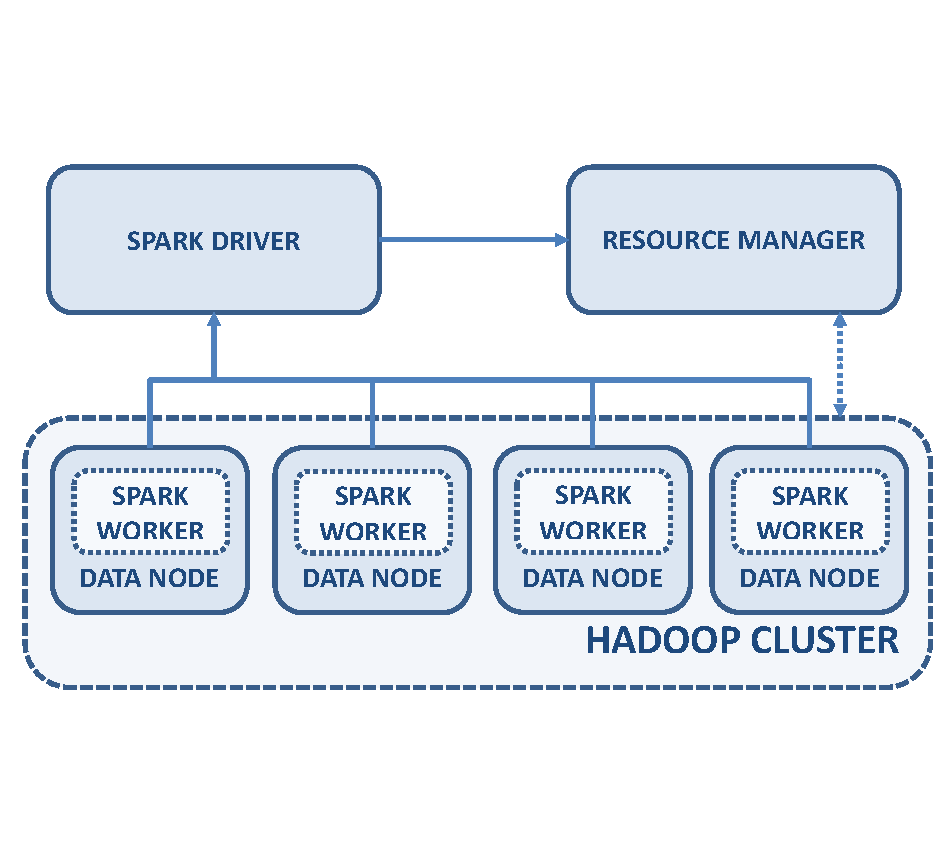
\includegraphics{BigData.pdf}
\caption{A basic illustration of a Hadoop architecture.}
\label{fig:BigData}
\end{figure}

The research community should consider pooling effort and resourcing to implement such architecture to facilitate cross-forge mining.
